\chapter{绪论}
\label{cha:intro}

\section{研究背景与意义}

脑机接口能够在不依赖外周神经和肌肉输出的条件下建立人脑与外部设备之间的信息通道，在神经康复、辅助交互、智能可穿戴和新型人机协同等方向具有重要应用价值 \cite{chaudhary2016brain, lotte2018review}。其中，基于脑电（Electroencephalography, EEG）的非侵入式脑机接口因采集成本较低、使用风险较小、便于重复实验和系统集成，成为当前研究与应用开发最活跃的技术路线之一。对于希望进入辅助交互与便携式使用场景的系统而言，安全性、可重复性与可集成性往往比单次实验中的极限性能更具现实意义，这也产生了面向真实应用条件构建无创脑机接口系统的研究需求。

\begin{figure}[htbp]
  \centering
  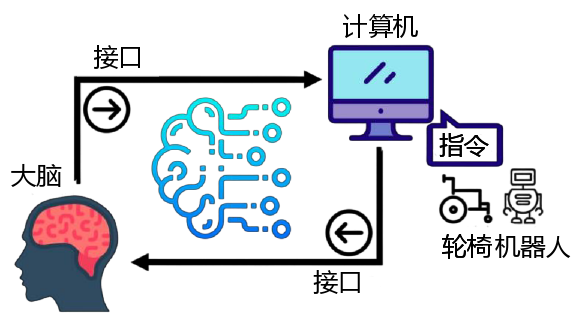
\includegraphics[width=0.75\textwidth]{figures/C1-1_BCI_system_and_apps.png}
  \caption{EEG-BCI系统的基本组成与典型应用场景示意\cite{gu2021eeg}}
  \label{fig:C1-1}
\end{figure}

如图\ref{fig:C1-1}所示，EEG-BCI系统通常由信号采集、预处理与特征提取、解码与控制以及应用终端等环节构成，其应用场景也已由实验室验证逐步扩展到康复辅助、交互控制与状态监测等方向。这种“从可测到可用”的演进进一步凸显了从系统链路角度开展研究的意义。

从任务范式看，脑电脑机接口已经形成了较为清晰的技术谱系。以 P300、稳态视觉诱发电位（Steady-State Visual Evoked Potential, SSVEP）和运动想象（Motor Imagery, MI）为代表的范式，分别对应事件相关模式检测、持续视觉刺激驱动识别和主动意图解码等不同交互路径 \cite{farwell1988talking, bin2011high, pfurtscheller1999event}。其中，运动想象无需真实肢体动作即可诱发可识别的感觉运动节律变化，也不依赖持续外部刺激维持，因此长期被视为主动控制类脑机接口中的典型范式；但与此同时，它对个体训练、状态稳定性和解码策略的依赖也更为突出。

从技术任务看，脑电解码大体围绕事件相关模式检测、脑状态分类识别以及连续意图或认知状态估计展开。面对这些不同的任务或范式，低信噪比和非平稳性始终是脑电解码的主要挑战：一方面脑电信号幅值较弱，易受肌电、眼电和环境噪声污染，整体信噪比较低 \cite{goncharova2003emg, lotte2018review}；另一方面已有研究表明，跨被试差异、跨 session 漂移以及试次级信号质量波动都会直接影响模型泛化与解码稳定性 \cite{lotte2018review, kwon2019subject, li2024joint, Zho16}，表现为脑电信号的非平稳性。

近年来，围绕上述难题，脑电解码研究持续从卷积网络深度、自注意力建模方式
以及训练数据规模等方向推进，同时也出现了面向跨被试迁移和表示复用的大规
模预训练模型。相关工作试图通过大规模跨数据集学习缓解异质性、样本不足和
泛化困难 \cite{Jia24, Wan24b}。例如，Jiang 等提出的
Large Brain Model for EEG 试图利用大规模跨数据集训练学习更通用的脑电表
征，以提升多任务场景下的迁移能力 \cite{Jia24}；Wang 等提出的 CBraMod
则进一步强调在不同 EEG 格式、不同任务和不同数据来源之间建立统一的表征空
间 \cite{Wan24b}。这类工作说明，大规模预训练和基础模型路线已经开始从单
一任务优化转向更广义的表示复用与跨域泛化。但现有综述也指出，这类路线的
主要优势仍集中于多导联、离线基准和较重适配条件下的表示迁移，其收益并不
能自动等同于低成本、少导联、实时交互和可部署系统中的直接可用性
\cite{Liu26b}。

随着辅助交互终端、可穿戴设备和日常化人机协同需求的发展，无创脑机接口系统正在逐步突破传统高密度有线实验平台的使用边界。一方面，市场上已经出现了以头环、头带和耳周设备为代表的轻量化 EEG 产品，相关产品多聚焦于睡眠监测、专注训练和基础认知调节等场景；另一方面，学术界也在持续探索耳电、前额阵列、低准备度无线采集和针对特定任务的可穿戴 EEG 系统 \cite{He23, Nis22, Arn20, Deb15, Bio22}。这表明，“更轻、更易用、更可持续部署”的 EEG 形态已经在市场探索和学术研究中形成可观察的发展方向，也进一步产生了围绕可穿戴实现、持续运行能力与部署可行性开展系统研究的现实需要。
从现有文献的证据强度看，这类轻量化形态的直接验证目前主要集中在睡眠监测、部分癫痫监测以及长时程日常化记录等任务上，因为这些任务与稀疏空间采样和长期佩戴条件具有较高匹配度；而面向更一般脑机交互目标的头环式、耳周式和眼镜式 EEG 形态则仍更多处于研究原型与场景探索阶段 \cite{Arn20, Deb15, Bio22, He23}。

但便携化、无线化和边缘化并不等同于对实验室设备进行简单的小型化改造。面向真实使用场景，系统往往需要同时兼顾穿戴便利性、布设时间、无线传输、持续运行、本地响应以及维护成本等多重要求 \cite{Cas19c, Nis22, He23}。在这种条件下，系统通常难以继续沿用实验室中的高密度有线配置，而需要围绕佩戴复杂度、部署成本与实时响应等因素重新组织采集与计算链路。相应地，采集端更可能采用简化导联配置和紧凑硬件实现，后端则必须在有限算力、有限存储和有限功耗预算下完成稳定推理。

由此带来的挑战可以概括为两个彼此关联的问题。首先，需要在受限采集与受限资源条件下同时兼顾解码模型的有效性、紧凑性与端侧部署友好性。在采集配置简化的条件下，系统可利用的空间观测通常更为有限，信号质量也更容易受到接触状态、运动伪迹、基线漂移和试次质量波动等因素影响。因此，相关研究不仅需要关注解码是否仍然可行，还需要进一步评估在有限算力和功耗预算下，何种任务目标与模型结构能够满足实际部署要求。同时，当系统进一步走向在线交互时，交互延迟、反馈机制和用户适应会继续改变任务表现，系统关注的重点也不再只是继续提高离线准确率，而是如何在真实使用条件下保持足够稳健、足够及时和足够可持续的交互能力。
此外，脑机接口面向真实应用的评价问题也并不能简单收敛为单一离线平均准确率。Thompson 等关于脑机接口性能度量的教程性综述指出，性能指标的选择应与具体使用模式和交互目标相匹配，仅凭单一分类分数往往难以完整反映系统的可用性与稳定性 \cite{Tho14}。Carrara 等进一步从伪在线评估角度表明，离线处理与伪在线/在线处理在时间窗组织、空闲状态建模和流式约束上存在实质差异，评价协议本身就可能改变算法表现与方法排序 \cite{Car23}。与此同时，Brookshire 等指出，不恰当的数据划分和信息泄漏会系统性夸大 translational EEG 研究中的测试结果，从而削弱离线高分对新被试和真实使用条件的参考价值 \cite{Bro24}。因此，对于面向辅助交互与便携式使用场景的无创脑机接口而言，评价重点还需要进一步扩展到协议设计、校准代价和真实交互条件下的稳健性。

\begin{figure}[htbp]
  \centering
  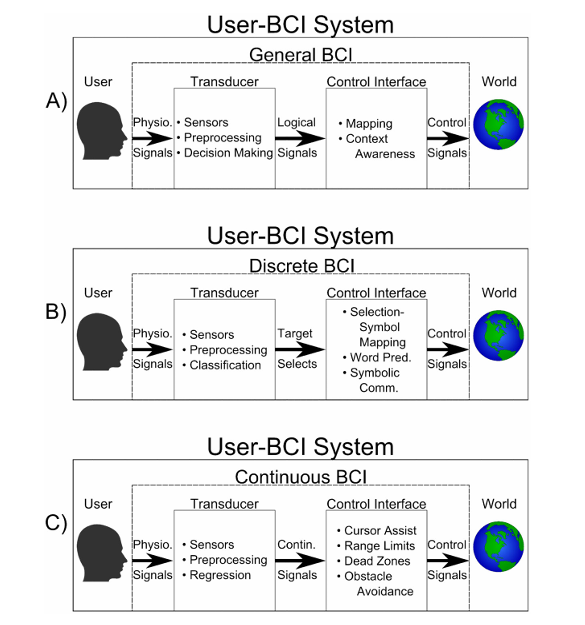
\includegraphics[width=0.8\linewidth]{figures/C1-4_BCI_modes_and_metrics.png}
  \caption{不同脑机接口使用模式下的系统组织差异\cite{Tho14}}
  \label{fig:C1-4}
\end{figure}

本课题以国家科技创新2030--“脑科学与类脑研究”重大项目《侵入式/非侵入式双向闭环脑机接口关键技术及系统》为背景，面向辅助交互与便携式使用场景下的无创脑机接口需求，以运动想象这一典型脑电交互任务为切入点，围绕真实应用中的系统实现与任务落地问题展开研究。结合前述分析，本文重点关注三个相互衔接的问题：其一，面向便携式与可持续运行需求，如何建立可用的双导采集、无线传输与基础交互链路；其二，在受限采集与受限资源条件下，标准高密度离线研究结论应如何收束为更适合真实系统的任务目标与解码方法；其三，离线算法主线如何进一步进入系统集成、模型更新与在线联动过程，并形成具有实际参考意义的初步验证。围绕上述问题，论文分别从双导采集硬件实现、面向低通道端侧场景的解码方法设计以及系统集成与在线联动初步验证三个层面展开工作，旨在建立从标准高密度设置到双导可部署方案的研究路径，为无创脑机接口在真实辅助交互场景中的应用提供参考。

\section{脑机接口系统与脑电采集研究现状}

围绕便携式实现、持续运行与本地响应等需求，脑机接口系统与脑电采集相关研究已经形成了较为清晰的技术脉络。现有工作大致可归纳为三个层面：一是围绕电极接口、模拟前端、模数转换、主控与通信模块展开的采集链路研究；二是围绕头环、耳周设备、前额阵列等形态展开的可穿戴系统研究；三是围绕嵌入式节点、量化压缩与链路协同展开的部署研究。这些研究共同构成了便携式脑机接口由“可采集”走向“可实现”的系统基础。

\subsection{脑电采集链路与硬件组成}

从系统实现角度看，脑机接口首先依赖稳定的脑电采集与处理链路。贺庆等对脑电采集设备硬件系统的综述表明，导联接口、预处理电路、模数转换电路、处理器、存储与通信模块以及供电模块共同构成了脑电采集系统的基本硬件框架，其中前端放大、滤波和参考方式直接影响微弱脑电信号的采集质量 \cite{He20}。更早的便携式采集芯片研究则开始将模拟前端、模数转换与数字控制集成到单芯片方案中，以支撑便携式 EEG 采集系统的低功耗实现 \cite{Martins98}。Kim 等进一步指出，可穿戴 EEG 的小型化并不只是器件体积压缩，还涉及记录硬件与数据处理链路的协同优化 \cite{Kim22wearable}。因此，对脑机接口系统的研究不仅涉及信号能否被采到，还涉及采集链路能否在有限体积、有限功耗和连续使用条件下稳定工作。

\begin{figure}[htbp]
  \centering
  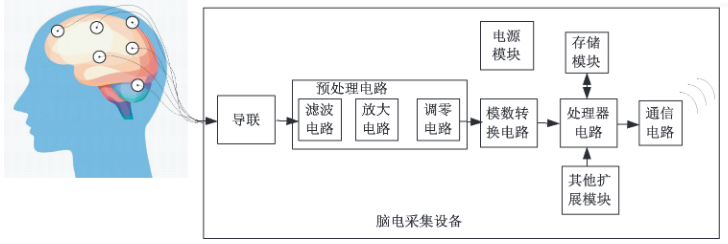
\includegraphics[width=0.88\linewidth]{figures/C1-2_EEG_acquisition_block_diagram.png}
  \caption{脑电采集设备的一般组成框图\cite{He20}}
  \label{fig:C1-2}
\end{figure}

围绕这一链路，现有研究大致沿两类硬件问题展开。首先，传统脑电采集设备研究重点关注前端放大、滤波、参考方式与高精度模数转换等关键环节，以提高微弱脑电信号采集时的共模抑制能力、输入阻抗和噪声控制水平 \cite{He20}。这类工作实际上奠定了后续脑机接口系统的共同技术底座，即无论系统最终是高密度实验平台还是轻量化原型，其前端都必须在高增益、低噪声、较强抗工频干扰和足够采样精度之间取得平衡。

其次，随着高集成模拟前端芯片和便携处理节点的发展，相关研究又进一步转向体积更小、功耗更低、便于无线回传的实现方案 \cite{Martins98, Kim22wearable}。这一变化的意义不只是硬件小型化本身，更在于它将“能否稳定采到脑电”与“能否在移动或连续使用场景下完成采集”联系起来。也正因如此，采集链路研究开始同时关注模拟前端集成度、无线连接方式、主控架构与供电设计，为后续可穿戴系统和嵌入式原型提供了更直接的工程参考。

\subsection{可穿戴形态与真实应用约束}

越来越多研究开始探索低准备度与可穿戴化的 EEG 形态，但不同形态往往对应不同任务与使用目标。Arnal 等将 Dreem 头环与多导睡眠监测进行比较，说明头环式轻量设备在特定睡眠分期任务中已经具备较有竞争力的信号采集与应用基础 \cite{Arn20}。Debener 等则展示了利用智能手机与耳周柔性电极实现非侵扰式 ambulatory EEG 的方案，强调耳周 EEG 在长时程、日常化记录中的隐蔽性与持续佩戴优势 \cite{Deb15}。面向癫痫监测场景，Biondi 等的系统综述进一步表明，移动化、减少导联的非侵入 EEG 已经形成较明确的临床与家庭应用需求，但也伴随着更强的任务依赖性和空间覆盖约束 \cite{Bio22}。
这些研究共同说明，可穿戴 EEG 的发展并不是沿着单一“更轻更小”的方向推进，而是在不同任务目标下形成分化的形态路线：头环和前额系统更强调低准备度与重复使用便利性，耳周和耳电系统更强调隐蔽性与长时佩戴能力，而临床导向的减少导联系统则更关注家庭或院外环境中的持续监测可行性 \cite{Arn20, Deb15, Bio22, He23}。

从真实应用约束的角度看，Casson 对 wearable EEG 的综述强调，离开实验室环境之后，系统设计目标会从尽可能完整的空间覆盖转向对舒适性、移动性和长期使用能力的综合权衡 \cite{Cas19c}。Niso 等对无线 EEG 系统的调查则进一步说明，无线传输、同步方式和移动场景下的使用条件已经成为系统设计不可忽略的组成部分 \cite{Nis22}。He 等对现有 wearable/wireless EEG 系统的多样性与适用性梳理表明，不同形态并非彼此替代，而是围绕具体任务、使用时长和部署条件形成不同折中 \cite{He23}。因此，可穿戴 EEG 的研究对象并不只是“更少的电极”或“更轻的设备”，而是对采集准备、使用方式与维护策略的整体重构。

\subsection{边缘节点与系统链路协同探索}

在系统级实现层面，已有研究开始将采集前端、无线链路与边缘算力节点放在同一框架下考察。Wang 等基于 EEGNet 的运动想象系统验证了低功耗边缘计算节点上完成脑电推理的可行性 \cite{Wan20}。Schneider 等进一步通过 8 bit 量化和平行实现，将 EEGNet 部署到 PULP 平台，强调了能效与推理速度之间的工程折中 \cite{Sch20}。En\'eriz 等则在 Arduino Nano 33 Sense 上实现了低功耗 EEGNet 脑机接口原型，说明更轻量的嵌入式平台也可以承担基础解码任务 \cite{Ene23}。此外，Wan 等通过通道选择与量化结合，展示了在压缩输入与模型规模后仍保持可接受解码表现的可能性 \cite{Wan22b}。这些工作说明，便携式脑机接口的系统研究已经不再停留在“设备能否采样”这一层面，而是进一步进入“采样之后如何在受限节点上完成稳定推理”的阶段。

\begin{figure}[htbp]
  \centering
  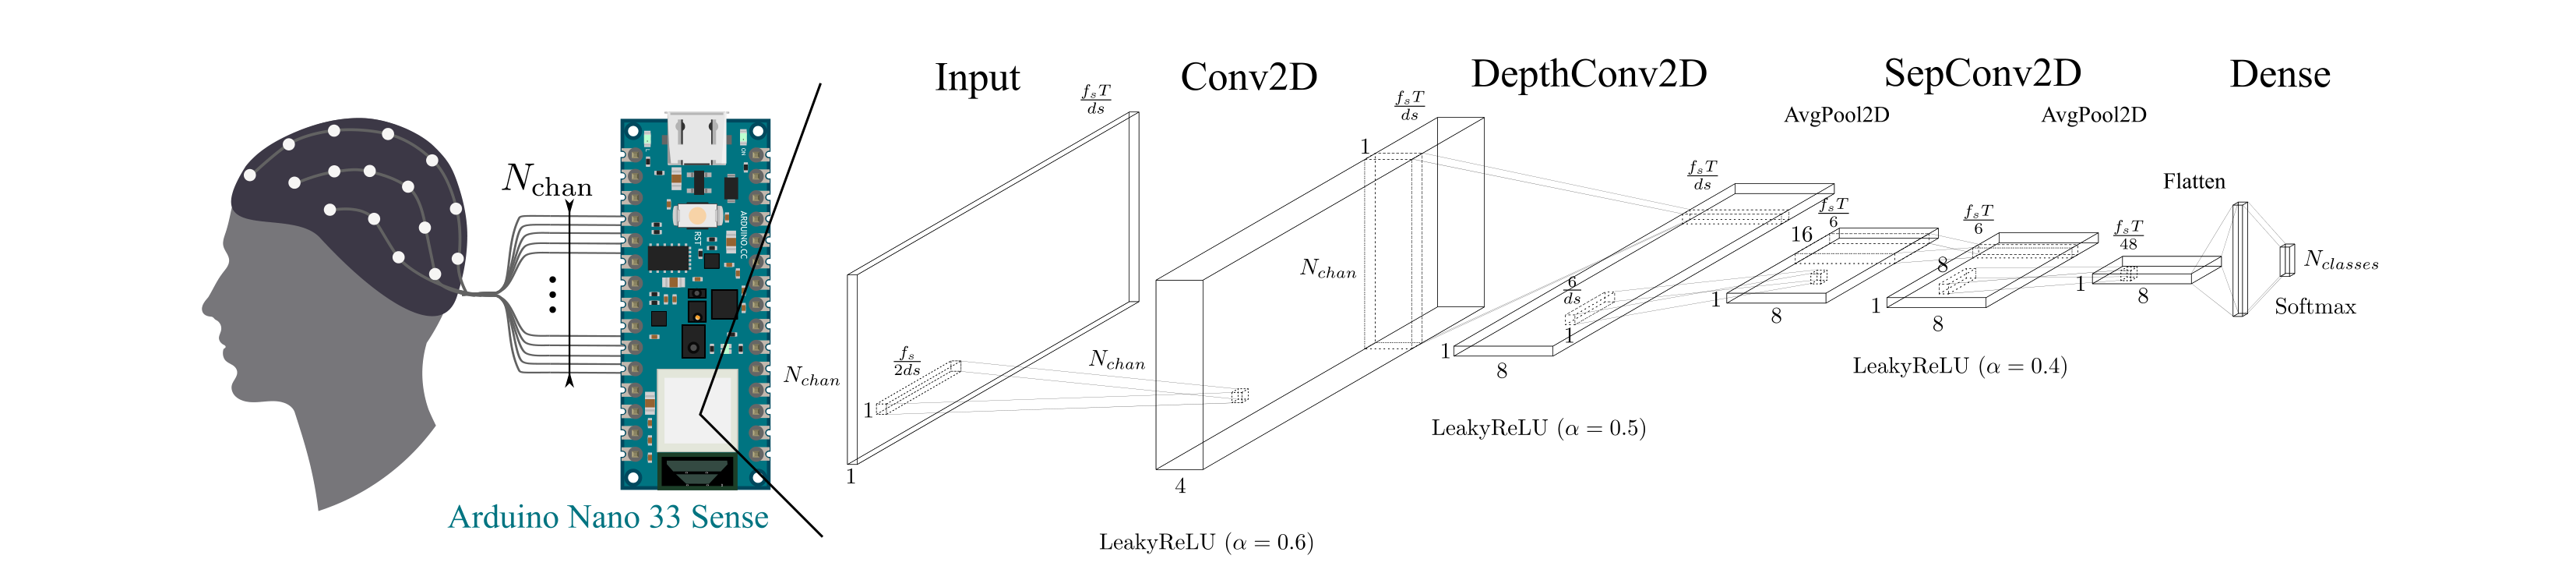
\includegraphics[width=\textwidth]{figures/C1-8_Edge_BCI_Prototype.png}
  \caption{基于嵌入式节点的轻量脑机接口原型与卷积网络部署示意\cite{Ene23}}
  \label{fig:C1-8}
\end{figure}

图\ref{fig:C1-8}展示了将轻量采集节点与紧凑卷积网络部署结合起来的原型思路。这类工作的重要意义不只在于证明模型“可以运行”，更在于说明采集形态、节点算力与网络结构已经开始被放在同一系统框架下联合考虑。

与此同时，部分相邻时序任务也开始围绕国产 SoC、NPU 或异构推理引擎开展优化。You 等在实时莫尔斯码解码任务中讨论了国产 SoC 上的本地实时处理能力 \cite{You24}；Ismagilov 则以目标检测为例评估了 Rockchip SoC 的推理性能边界 \cite{Ism23}。尽管这些结果并不能直接替代脑电场景中的端到端实测，但它们至少说明，围绕采集、传输、推理和交互节点进行整体化协同已经成为系统研究的重要方向。现有证据也由此表明，采集配置、链路时序和推理节点之间存在明显耦合关系，系统设计需要在这些因素之间进行联合权衡，而不能仅围绕单一局部环节开展优化。

总体来看，现有研究已经从采集链路、可穿戴形态和部署节点三个层面证明了便携式脑机接口的基本可行性，并为后续双导硬件与端侧原型设计提供了重要视野。然而，多数工作仍主要回答某一局部问题，例如前端是否足够低噪声、设备是否更易佩戴，或模型能否在指定节点运行；对于真实辅助交互场景下究竟应采用何种采集配置、何种系统链路以及何种任务组织方式，仍缺少统一而连续的研究路径。

\section{脑电解码方法研究现状}

从方法演进看，脑电解码研究已经形成了较为清晰的技术谱系。对于运动想象脑电这一典型任务而言，现有工作既追求更高的离线分类性能，也越来越重视在跨被试、跨会话和真实使用约束下的泛化能力与可用性。从完整分析链条看，相关研究通常围绕信号预处理、特征提取与表示学习以及分类识别三个关键环节展开；若从建模思路进一步划分，当前方法又大致可以归纳为传统特征工程与浅层分类、卷积神经网络与紧凑深度模型、自注意力与 Transformer 结构，以及预训练、迁移与在线适配增强等几条彼此衔接的路线。

\subsection{信号预处理方法}

脑电解码中的信号预处理主要目标是提升有效神经活动的可观测性，并尽量削弱采集过程中的噪声、伪迹与非任务相关波动。对于运动想象任务而言，预处理虽然通常位于分析流程的前端，但它并非单纯的“数据清洗”步骤，而是会直接影响后续特征分布、判别边界和模型稳定性。因此，经典脑电分析流程往往将预处理视为与特征提取和分类识别同等重要的基础环节 \cite{lotte2018review}。

从技术组成看，预处理方法大致包括四类。第一类是空间参考与空间滤波，其目的在于利用多通道之间的空间关系抑制共模噪声并增强目标模式，其中共同平均参考（CAR）是最常见的基础方法之一 \cite{offner1950eeg}。第二类是时域与频域滤波，通常通过带通滤波保留与任务相关的 $\mu$、$\beta$ 等节律范围，通过陷波滤波抑制工频干扰，并结合高通滤波降低基线漂移对后续分析的影响 \cite{picton2000guidelines}。第三类是伪迹检测与抑制，主要面向眼电、肌电、心电以及突发性运动伪迹等非神经成分，相关方法从振幅阈值、小波分析发展到基于 ICA 或信号重建的去伪迹方案，目标是在保留有效脑电模式的同时降低污染数据对解码结果的干扰 \cite{sweeney2012artifact, albera2012ica}。第四类则是标准化与基线校正，包括幅值归一化、基线扣除以及在必要时进行空间插值或布局对齐，以增强不同试次、不同被试和不同采集条件下数据的可比性 \cite{lotte2018review}。

这些预处理策略为传统脑电分析和早期脑机接口系统奠定了方法基础，其价值在今天仍然存在：即便后续建模已经逐步转向深度学习和自注意力结构，带通滤波、参考重构、伪迹处理和标准化等步骤仍然决定着输入信号的统计特性，并在很大程度上影响模型能否学习到稳定可靠的时空表示。因此，后续不同解码路线虽然在特征表示和分类器结构上差异明显，但在预处理阶段大多仍沿用上述经典思想，并围绕特定任务做适配调整。

\subsection{传统特征工程与浅层分类路线}

早期运动想象脑电解码主要依赖人工特征与浅层分类器。以共空间模式（Common Spatial Pattern, CSP）及其滤波器组扩展方法（Filter Bank CSP, FBCSP）为代表的空间滤波路线，能够突出不同类别在空间方差分布上的差异，并与线性判别分析（LDA）、支持向量机（SVM）等浅层分类器结合取得较高分类效率 \cite{ang2012filter, lotte2018review}。这类方法的核心优势在于实现简单、计算代价较低、可解释性较强，因此至今仍是运动想象任务的重要比较基线。

不过，传统特征工程路线的优势也伴随着较强的先验依赖。其性能通常与频带选择、时间窗划分、人工特征设计以及相对稳定的采集条件密切相关，因此在跨被试迁移、复杂噪声场景与长期在线使用条件下存在明显边界。正因如此，后续深度学习研究才逐步从“如何设计更好的人工特征”转向“如何由模型自动学习更稳定的时空表示”。

\subsection{卷积神经网络与紧凑深度模型路线}

为减少对手工特征工程的依赖，卷积神经网络逐步成为脑电解码的重要技术路线。Schirrmeister 等提出的深浅卷积网络说明，端到端学习方式能够直接从原始脑电片段中提取具有判别性的时空特征 \cite{schirrmeister2017deep}；Lawhern 等提出的 EEGNet 进一步通过紧凑型卷积结构在较低参数规模下兼顾跨范式适应能力与部署友好性 \cite{lawhern2018eegnet}。此后，多分支卷积、时频联合卷积等变体持续出现，其共同特点是在保留局部时空建模能力的同时，尽量控制参数量与推理复杂度。

\begin{figure}[htbp]
  \centering
  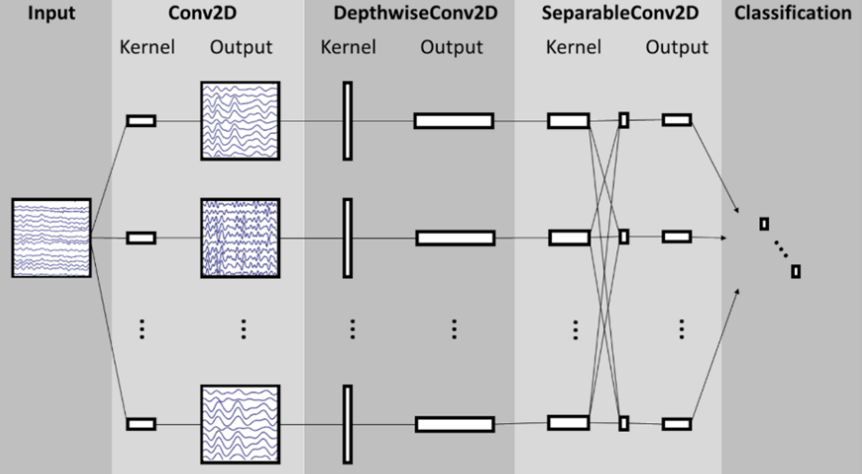
\includegraphics[width=0.75\linewidth]{figures/C1-3_EEGNet_architecture.png}
  \caption{EEGNet 紧凑卷积结构示意\cite{lawhern2018eegnet}}
  \label{fig:c1_3_eegnet}
\end{figure}

这一路线推动脑电解码由人工特征设计转向自动表示学习，也为后续端侧友好建模提供了重要基础。尤其是 EEGNet 这类紧凑模型，其价值并不只是“参数更少”，还在于它为脑电任务提供了一种兼顾局部时序滤波、空间滤波和较低部署成本的统一结构。也正因如此，卷积紧凑模型在后续受限采集和边缘部署研究中长期被视为重要起点。

\subsection{自注意力与 Transformer 路线}

在 CNN 基础上，Transformer 及其变体被进一步引入脑电解码领域，以增强对长程时序依赖和跨特征关联的建模能力 \cite{vaswani2017attention}。Song 等提出的 EEG Conformer 通过卷积与自注意力协同提取局部时空特征和全局时间依赖 \cite{songEEG2022}，Xie 等展示了 Transformer 结构在原始脑电分类任务中的应用潜力 \cite{xie_transformer-based_2022}。这些工作推动了脑电解码从局部卷积主导的建模方式，转向同时关注长程依赖和跨特征关系的时序建模框架。

\begin{figure}[htbp]
  \centering
  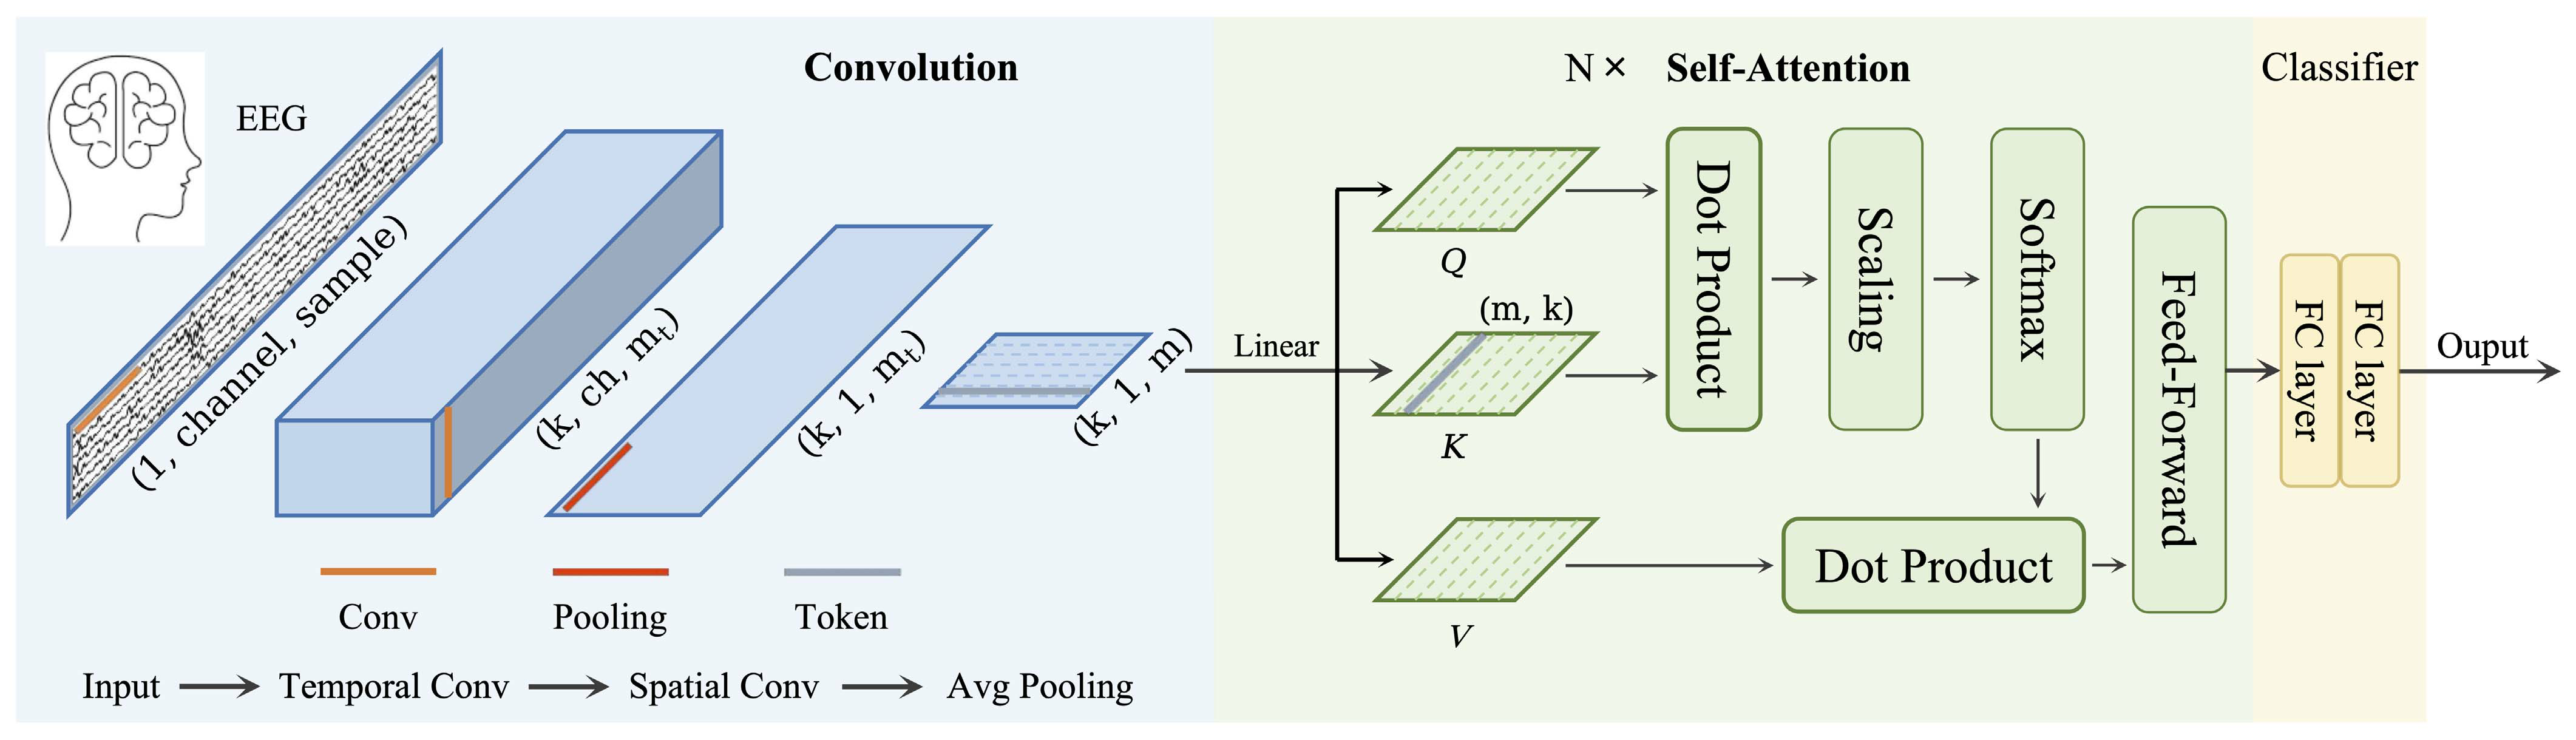
\includegraphics[width=0.92\linewidth]{figures/C1-5_EEG_Conformer_architecture.png}
  \caption{EEG Conformer 卷积与自注意力协同解码的框架示意图\cite{songEEG2022}}
  \label{fig:C1-5}
\end{figure}

如图\ref{fig:C1-5}所示，EEG Conformer 将卷积模块、自注意力模块与分类器串联起来，先利用时间卷积和空间卷积提取局部时空表征，再利用自注意力模块建模更长程的时间依赖。这种“卷积提取局部结构、注意力补充全局关联”的组合方式，为后续围绕端侧友好性开展结构改进提供了直接参考。

随后，研究重点又从“能否使用自注意力”转向“如何在控制复杂度的同时保留关键建模能力”。例如，Wan 等将通道注意力与窗口化机制结合建模时空耦合信息 \cite{wan2023novel}，Hua 等通过卷积与滑动窗口注意力的协同设计增强多尺度特征建模能力 \cite{hua2023improved}，Keutayeva 等则进一步强调了紧凑型结构在跨被试任务中的部署潜力 \cite{keu2024compact}。这表明，自注意力路线已从单纯追求更强表达能力，逐步转向更加关注高效性、紧凑性与可部署性，也因此与本文后续的方法设计形成了直接关联。

\subsection{预训练、迁移与在线适配增强路线}

近年来，围绕异质性、样本不足和泛化困难，预训练与大规模表示学习开始成为脑电解码研究的新方向。相关工作试图通过大规模跨数据集学习缓解跨被试差异、标注稀缺和表示复用问题 \cite{Jia24, Wan24b}。例如，Jiang 等提出的 Large Brain Model for EEG 试图利用大规模跨数据集训练学习更通用的脑电表征，以提升多任务场景下的迁移能力 \cite{Jia24}；Wang 等提出的 CBraMod 则强调在不同 EEG 格式、不同任务和不同数据来源之间建立统一的表示空间 \cite{Wan24b}。这类研究说明，脑电解码方法的前沿探索已不再局限于单一数据集或单一任务，而是开始尝试构建更一般化的表示学习框架。

与此同时，在线研究持续指出，仅靠更强的离线表征并不足以直接解决实际交互问题。Pfurtscheller 等和 Neuper 等的早期研究已经表明，反馈训练会显著影响左右手感觉运动节律的可分辨性 \cite{Pfu97, Neu99}；Meng 等进一步将导联数量、算法结构和长期训练表现放在统一框架下考察，说明紧凑通道方案在合理任务设计下仍可获得具有竞争力的在线表现 \cite{Men18}。因此，解码方法的有效性并不完全由离线模型结构决定，表示迁移、用户训练、校准代价和系统链路都会改变最终表现。现有综述也指出，预训练与大模型路线的主要优势仍集中于多导联、离线基准和较重适配条件下的表示迁移，其收益并不能自动等同于受限采集和在线交互系统中的直接可用性 \cite{Liu26b}。

总体来看，脑电解码方法已经形成了从传统空间滤波、卷积建模到自注意力结构，再到预训练与在线适配增强的清晰演进路径，并在标准数据集上不断提升分类性能。然而，现有证据仍主要建立在离线、标准协议和相对高密度导联条件之上，关于这些方法在真实系统约束下如何完成任务收束、结构压缩与在线协同，仍缺少更统一的回答。这也正是后续不足分析与本文研究路线需要进一步展开的部分。

\section{现有研究存在的不足}

第~1.1 节已经表明，面向辅助交互与便携式使用场景的无创脑机接口研究，不再只关心实验室条件下的单次解码性能，而是进一步产生了对可穿戴实现、无线传输、持续运行、本地响应和稳定交互能力的综合需求。结合第~1.2 节和第~1.3 节可以看到，现有研究虽然分别在系统形态、采集链路、解码方法和在线适配等方面积累了较多成果，但围绕这些需求仍存在三个相互衔接的不足。

第一，围绕便携式与可持续运行需求的系统级回答仍然不够完整。现有工作已经证明低噪声采集前端、可穿戴 EEG 形态和嵌入式推理节点分别具有实现基础，但多数研究仍聚焦于某一局部环节，例如前端噪声控制、设备佩戴便利性或指定节点上的模型运行。相较之下，真实辅助交互场景更需要统一回答采集配置、无线链路、基础交互方式和持续运行条件如何协同设计，以及何种系统组织方式能够在可实现性与可用性之间取得平衡。

第二，围绕受限采集与受限资源条件的任务收束与方法选择仍缺少统一路径。现有脑电解码研究已经形成了从传统特征工程到卷积网络、自注意力结构再到预训练与在线适配增强的清晰演进路线，并在标准数据集上持续提升离线性能。然而，这些结论主要建立在标准协议和较高导联配置之上，对真实系统中更受限的采集条件并不一定能够直接给出等价回答。当前研究仍较少系统说明：在空间观测更有限、资源预算更严格的条件下，应如何重估原有任务目标，如何在模型有效性、结构紧凑性与端侧部署友好性之间进行联合取舍，以及如何建立相应的定量证据链。

第三，围绕系统集成、模型更新与在线联动的验证证据仍然相对薄弱。已有研究已经指出，反馈训练、试次质量、跨会话漂移以及评价协议本身都会改变系统表现，离线高分并不能自然等同于真实交互中的稳定收益。但从公开研究看，关于离线算法主线如何进一步进入系统集成过程、如何通过轻量模型更新适应个体与轮次变化、以及如何在在线或准在线条件下形成具有参考意义的验证证据，仍缺少更连续的系统性研究。尤其对于面向便携式使用的原型系统而言，采集链路噪声、BLE 传输时序、交互延迟与校准代价往往同时影响最终可用性，这些因素尚未被充分纳入统一分析。

因此，现有研究虽然为本文提供了系统实现、方法设计和在线探索的多方面基础，但在系统级约束分析、任务与方法收束以及在线联动验证三方面仍留有明显空白。围绕这些不足，本文进一步从双导采集硬件、端侧友好解码方法以及系统集成与在线联动初步验证三个层面展开研究。

\section{本文主要研究内容与技术路线}
\subsection{主要研究内容}

围绕上述问题，本文面向辅助交互与便携式使用场景下的无创脑机接口系统，开展了以下几方面研究工作。

（1）设计并实现双导脑电采集硬件系统。针对辅助交互与便携式使用场景下的双导采集需求，本文完成了以双导联采集为核心的硬件系统设计与实现，构建了脑电前端、主控、BLE 回传和上位机交互的基础链路，并通过节律验证、标签链路验证和通信稳定性测试，为后续在线实验提供系统基础。

（2）研究面向受限采集与端侧部署条件的改进型自注意力脑电解码方法。针对标准条件下形成的高密度解码模型难以直接迁移到实际系统的问题，本文设计了兼顾局部时序建模能力、复杂度控制与部署友好性的改进型自注意力解码方法，在标准条件下完成性能、复杂度与量化友好性分析，并为后续方法落地提供算法基础。

（3）研究标准离线结论向可部署任务目标与解码路径的收束方法。围绕真实系统中受限采集与有限资源的特点，本文分析运动想象脑电任务在采集配置简化条件下的目标设定与方法适配问题，形成与双导系统相匹配的解码主线，使后续系统实现与在线验证建立在更合理的任务设定之上。

（4）完成双导端侧系统集成与在线联动初步验证。本文以双导硬件为前端、以上位机和可扩展推理节点为原型载体，构建了预训练初始化、轮次级模型更新与跨轮次判别反馈的在线联动机制，并结合伪在线评估和真实在线试跑，对系统的可实现性进行了初步验证。需要指出的是，当前实验阶段的在线验证载体主要为 Linux PC 原型环境，后续目标部署节点则面向 RK3568 / RKNN 一类嵌入式平台。

\subsection{技术路线与论文组织}

全文的技术路线与组织结构如图\ref{fig:org}所示。
\begin{figure}[htbp]
  \centering
  % \includegraphics[width=0.8\textwidth]{org_structure}
  \caption{论文技术路线与组织结构}
  \label{fig:org}
\end{figure}

本文后续各章安排如下：

第 2 章介绍运动想象脑电解码与端侧系统实现所需的关键技术基础，并在比较可选技术路线的基础上说明本文采用的建模与部署路线。

第 3 章围绕双导脑电采集硬件系统的设计与实现展开，重点说明采集前端、主控、无线通信和基础链路验证结果。

第 4 章研究面向低通道端侧场景的改进型自注意力脑电解码方法，在标准条件下建立离线基线，并进一步讨论受限采集条件下的任务收束与模型适配问题，为双导系统中的方法落地提供依据。

第 5 章进一步将第 4 章得到的低通道解码主线映射到双导系统中，介绍系统集成、在线实现机制、伪在线评估以及真实在线初步验证结果。

第 6 章对全文工作进行总结，并围绕更强的人机协同、自适应学习和更自然的实验范式给出后续展望。
